\begin{frame}
\frametitle{Needle in a haystack problems}

\begin{columns}[T] % align columns

\begin{column}{.50\textwidth}
\begin{figure}[htbp]
\begin{center}
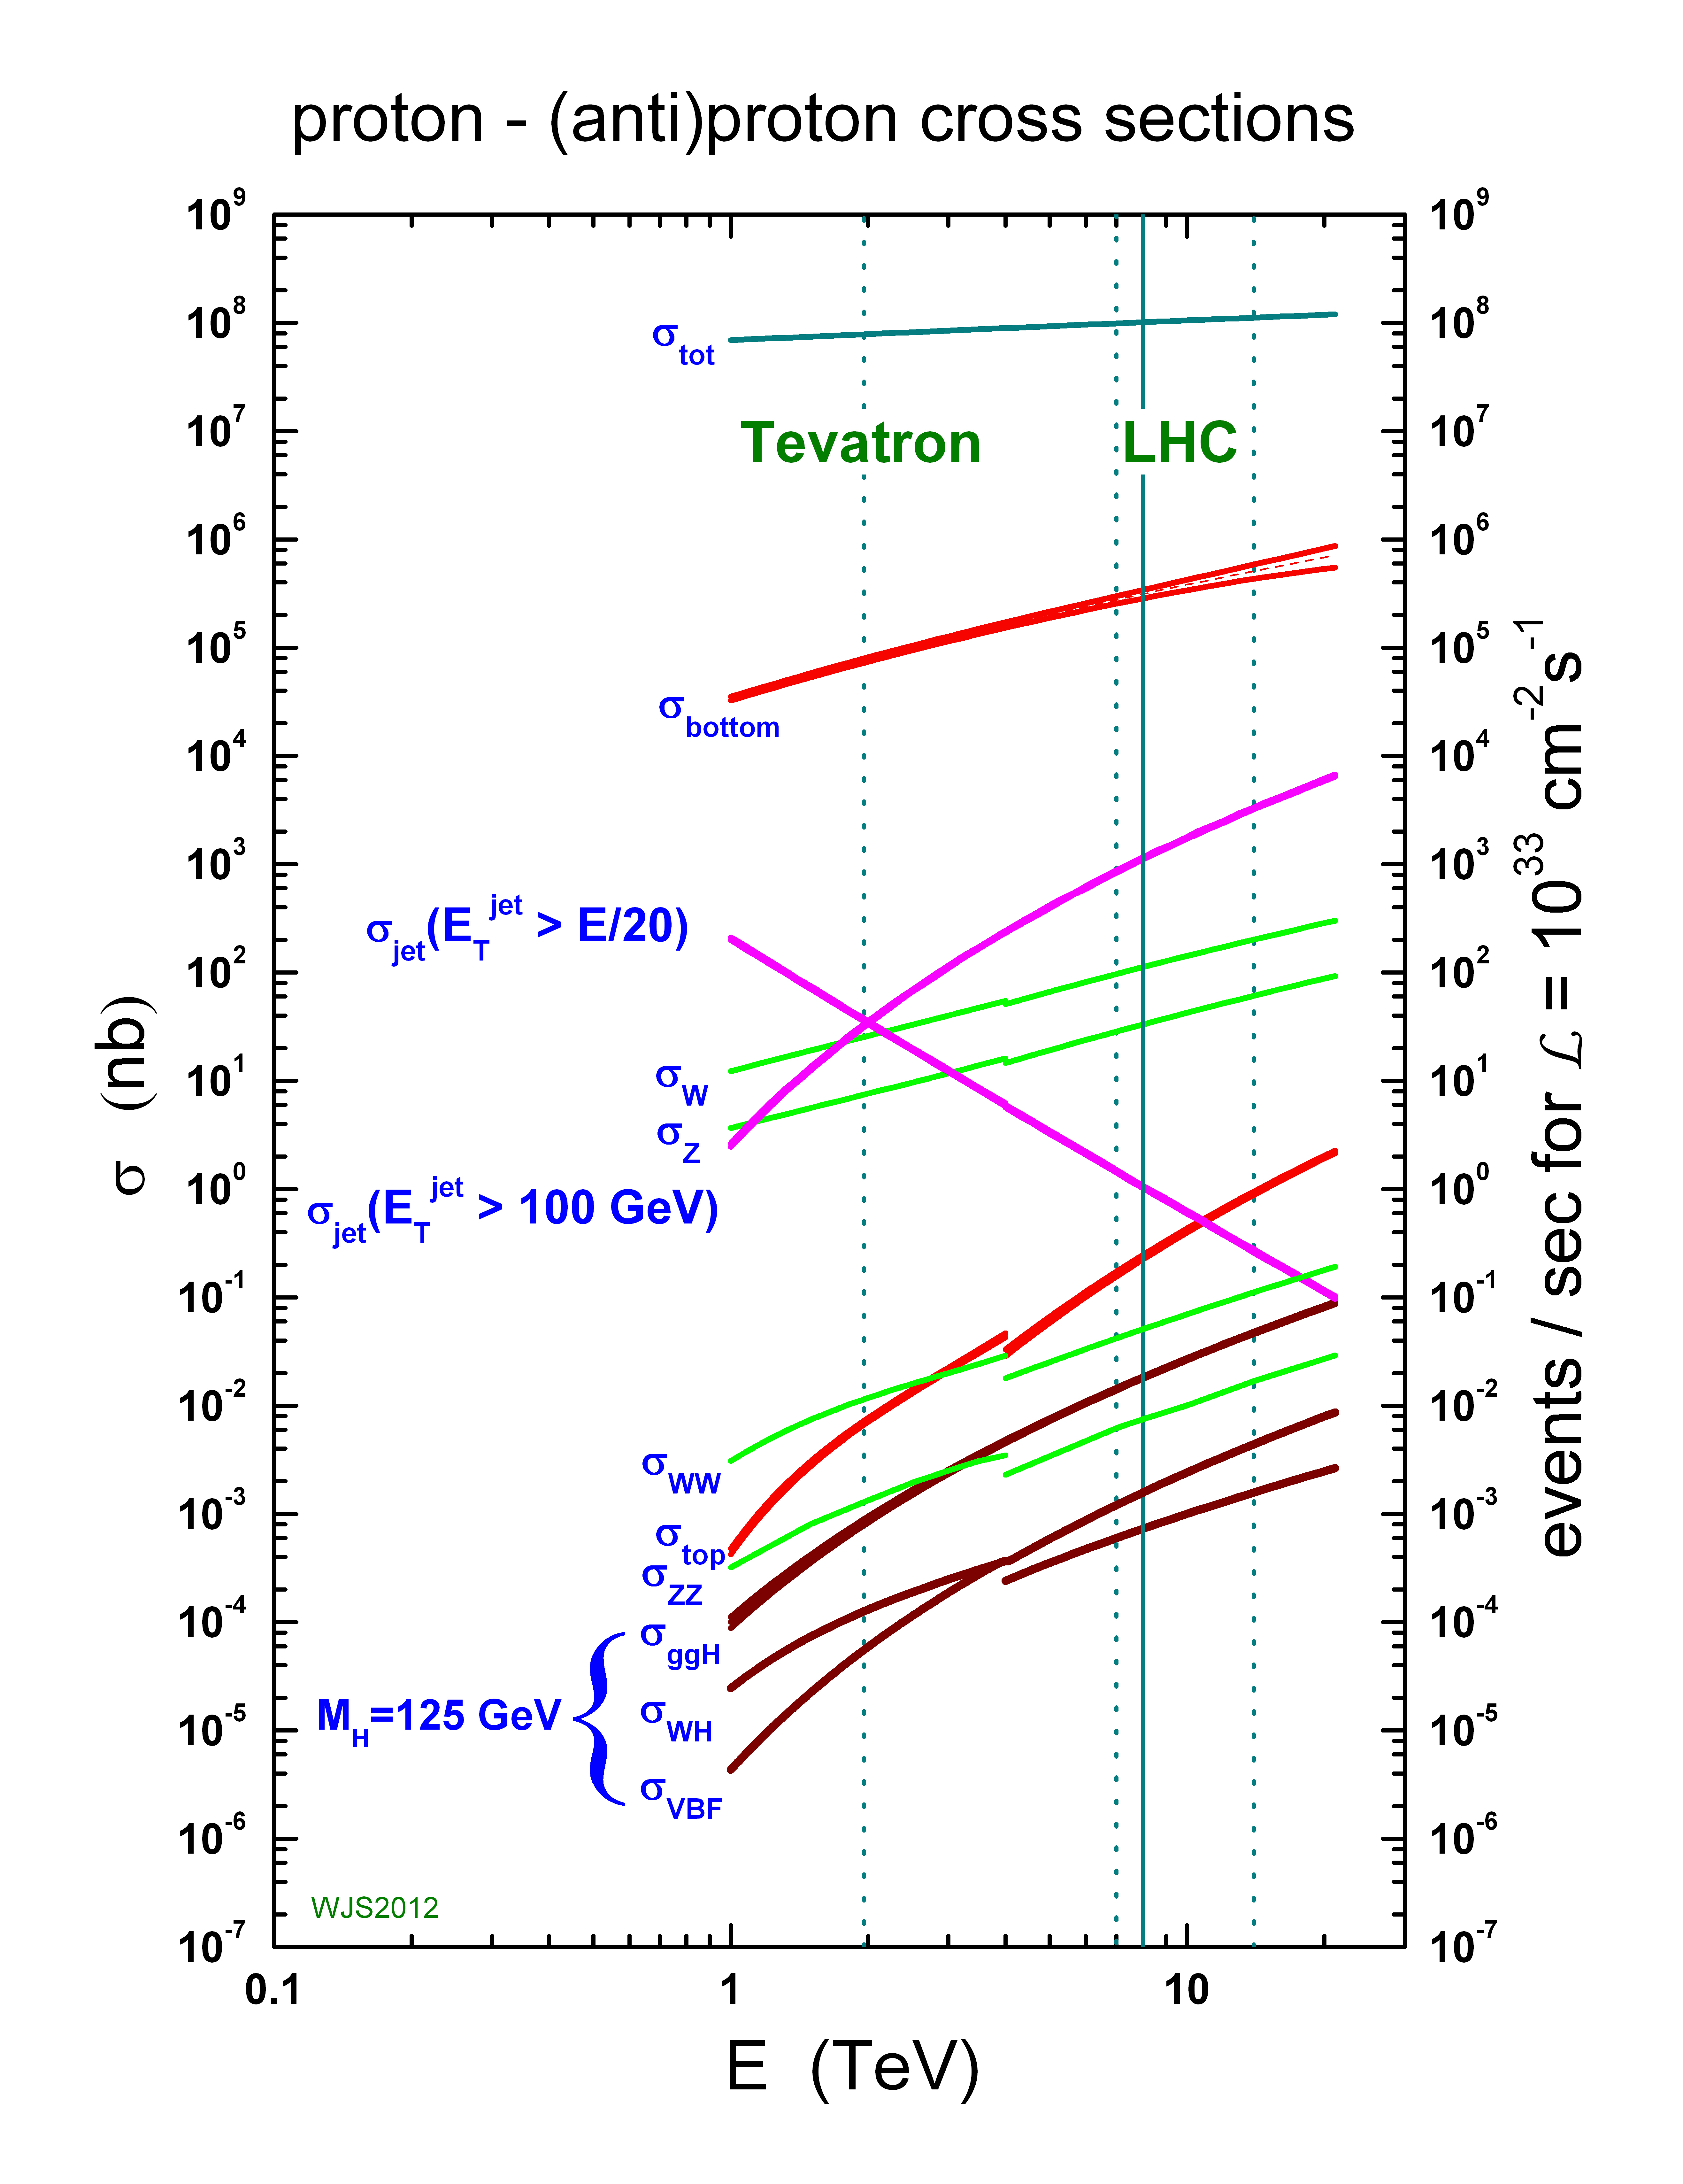
\includegraphics[width=0.9\textwidth]{images/crosssections2013.jpeg}
%\caption{}
%\label{fig:example2}
\end{center}
\end{figure}
\end{column}%

\begin{column}{.50\textwidth}
\vskip 0.5in
\begin{itemize}
\item Show is the production rates for various processes versus center-of-mass energy of collisions
\item Orders of magnitude difference between signal and background
\item Colliders have two ``knobs'': the energy and the ``luminosity'' (intensity) of collisions
\end{itemize}
\end{column}%




\end{columns}

%\small{Example Text}

\end{frame}


